\documentclass[10pt,a4paper]{article}

%\usepackage{lipsum}
%\usepackage{here}
%\usepackage{qtree}

%\usepackage{amstext}
%\usepackage{multirow}
%\usepackage{subfigure}
%\usepackage{algorithm}
%\usepackage{algorithmic}
%\usepackage{listings}
%\usepackage{xcolor}

\usepackage{verbatim}
\usepackage{url}
\usepackage{amsmath}
\usepackage[UKenglish]{isodate}
\usepackage{graphicx}
\usepackage{multicol}
\usepackage{caption}
\usepackage{multicol}
\usepackage[margin=0.67in]{geometry} %margins usually 0.67

\begin{document}

\title{Galaxy Survey}
\author{Aidan  Boxall}
\maketitle

\begin{abstract}
The aim of this investigation was to produce a catalogue of galaxies from an image taken by the Spitzer Space Telescope. From this catalogue the number of galaxies were plotted against apparent  magnitude to see if the relationship matched that expected if the galaxies were uniformly distributed with a given flux distribution. The relationship between galaxy population and flux density was found to be similar but not entirely consistent with the predicted relationship. A number of possible explanations are considered but the most likely explanation is that the discrepancies are due to the small sample size of galaxies investigated.
\end{abstract}

\section*{Introduction}
The aim of this investigation was to produce a catalogue  of galaxies from the image shown in Figure \ref{mosaic} taken by the Spitzer Space Telescope. The catalogue  produced includes the position, count and magnitude of the galaxies in the image. The catalogue  was produced using a python script. A number of different algorithms were investigated to determine the number of galaxies and their counts. 
 \begin{center}
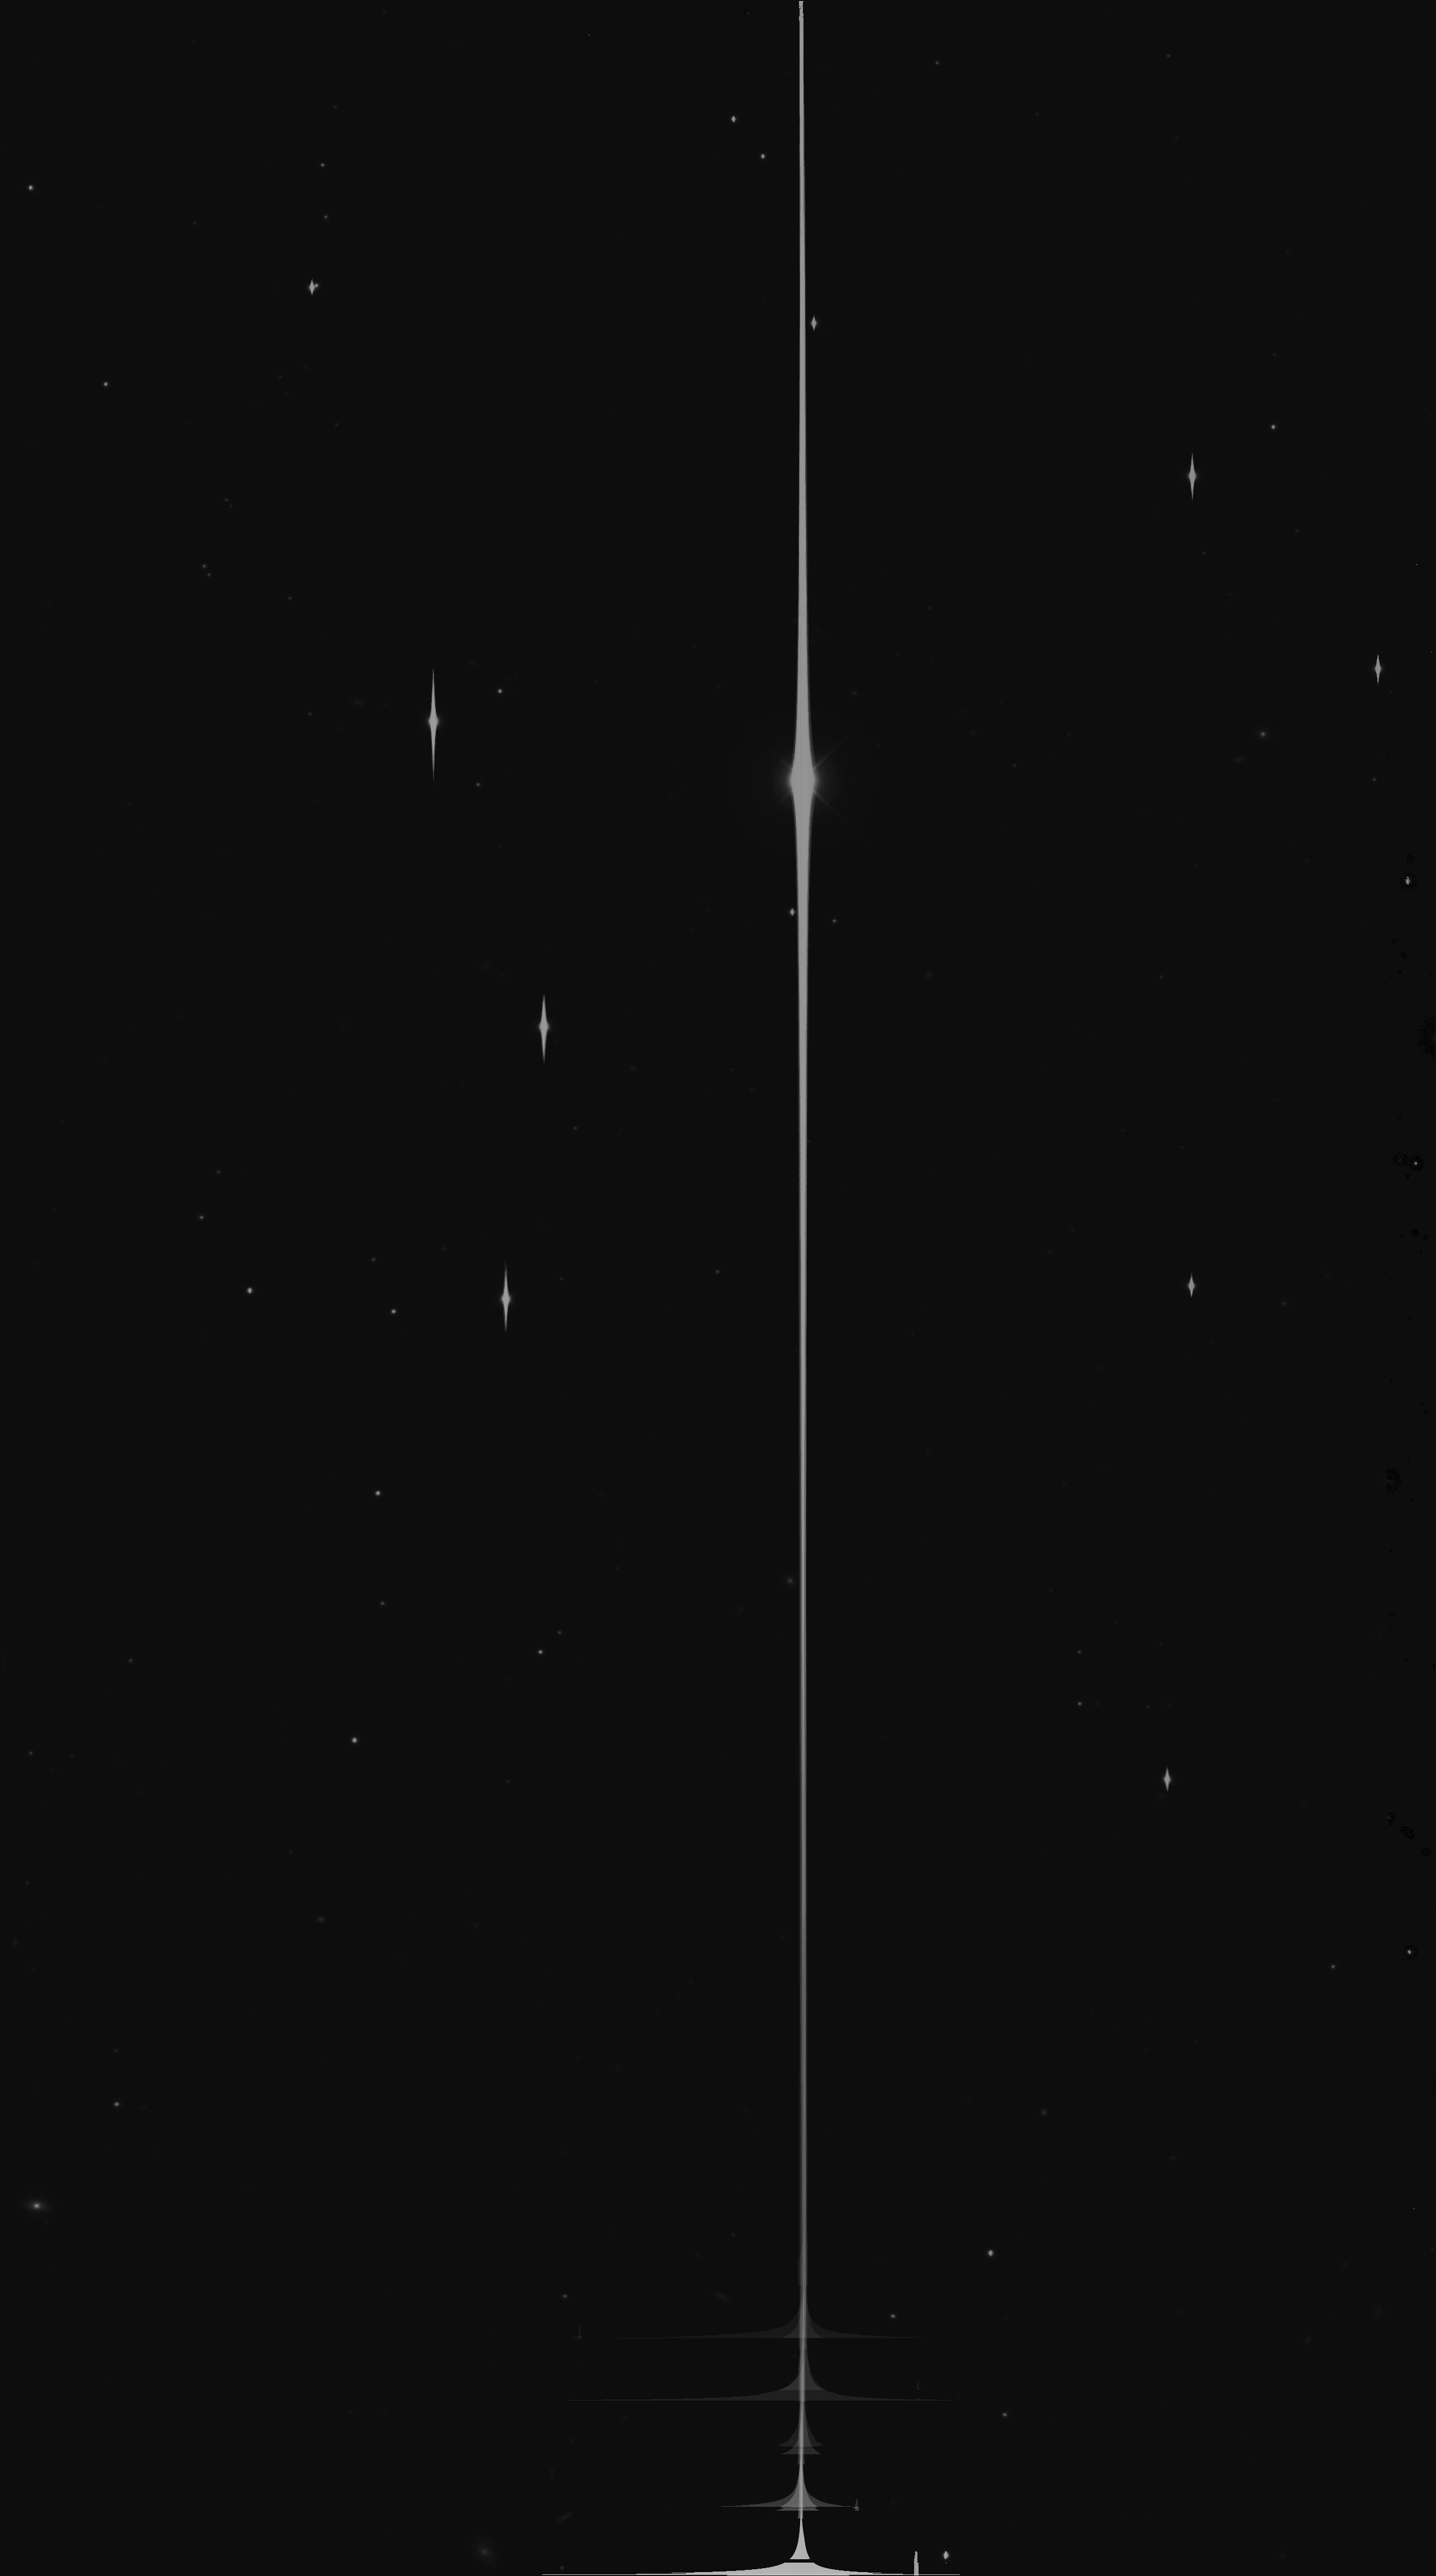
\includegraphics [width=5 cm]{mosaic.png}
\captionof{figure}{The image used as the data source for this investigation.}
\label{mosaic}
\end{center}
The galaxy magnitudes were used to investigate the relationship:
\begin{equation} \label{eq:main}
\log(N(m)) = 0.6m + constant
\end{equation}
where N(m) is the number of galaxies below an apparent magnitude $m$. This relationship was derived by making several assumptions about galaxies. It assumes a uniform distribution of galaxies with a given distribution of flux and uniform density. A full derivation can be found in the appendix.

The image was taken using a charge coupled device (CCD) camera. A CCD produces pixel counts which are linearly related to the number of photons absorbed by the device \cite{lab_script}. This makes it straightforward to locate the brightest points in the image and find an average background count.

\section*{Experimental Method}
\subsection*{Background Count}
The first aim of the experiment was to find a measure of the background count. The background count was needed for two reasons. Firstly it was necessary as it gave a lower limit to the pixel count that could be considered a galaxy. The minimum pixel count of a galaxy was determined by the average background count plus a number of standard deviations. The number of standard deviations to use was determined experimentally to be five. This gave the best compromise between not discarding too many galaxies with low counts and not counting background noise as galaxies. The background count was found by producing a histogram of all the pixel counts in the image, which is shown in Figure \ref{whole hist}. From this histogram a peak could be seen in the low count range corresponding to the background. A second histogram shown in Figure \ref{hist} was produced focusing on this region. The mean and standard deviation of the background count were calculated and a Gaussian distribution with the same mean and standard deviation is shown in Figure \ref{hist}. This shows that the background noise is approximately Gaussian distributed.

\begin{center}
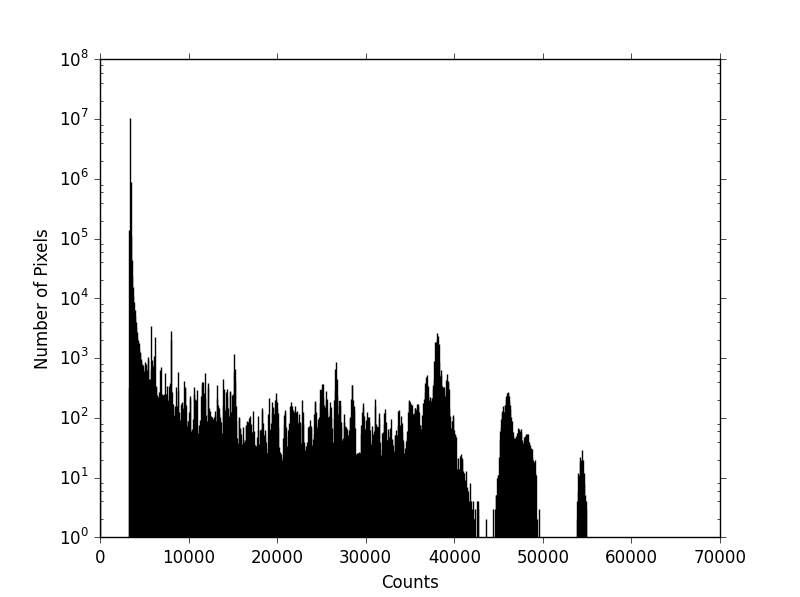
\includegraphics [width=10 cm]{whole_hist.png}
\captionof{figure}{A histogram of the pixel values of the entire image. There is a clear peak at around 3500 counts which corresponds to the background noise in the image.}
\label{whole hist}
\end{center}

\begin{center}
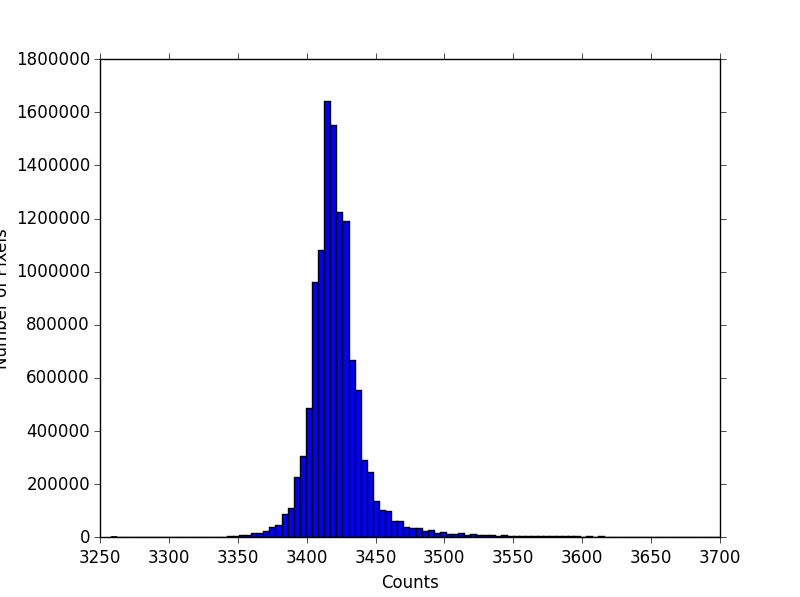
\includegraphics [width=10 cm]{hist.png}
\captionof{figure}{A histogram of the background noise pixel counts.}
\label{hist}
\end{center}

\subsection*{Masking Stars and Fixing Dead Pixels}
Once the background count had been determined the next stage was to determine an algorithm for cataloging galaxies. Galaxies were located by successively finding the brightest pixel in the image, taking counts within a circular aperture around the pixel and then marking that galaxy as counted in a mask image. This method required the stars and bleed pixels to be masked out so that they would not be counted as galaxies. Bleed pixels occur when a bright source causes a cell in the CCD to overflow with electrons into neighboring pixels \cite{lab_script}. The stars and surrounding bleed pixels were found by eye and masked as shown in Figure \ref{mask}. The image also contained a number of dead pixels, pixels with a count of zero. These were potentially problematic as if they were included in a galaxy count they would make the count lower than it should be. These pixels were dealt with by replacing them with the average count of the neighboring pixels. 

 \begin{center}
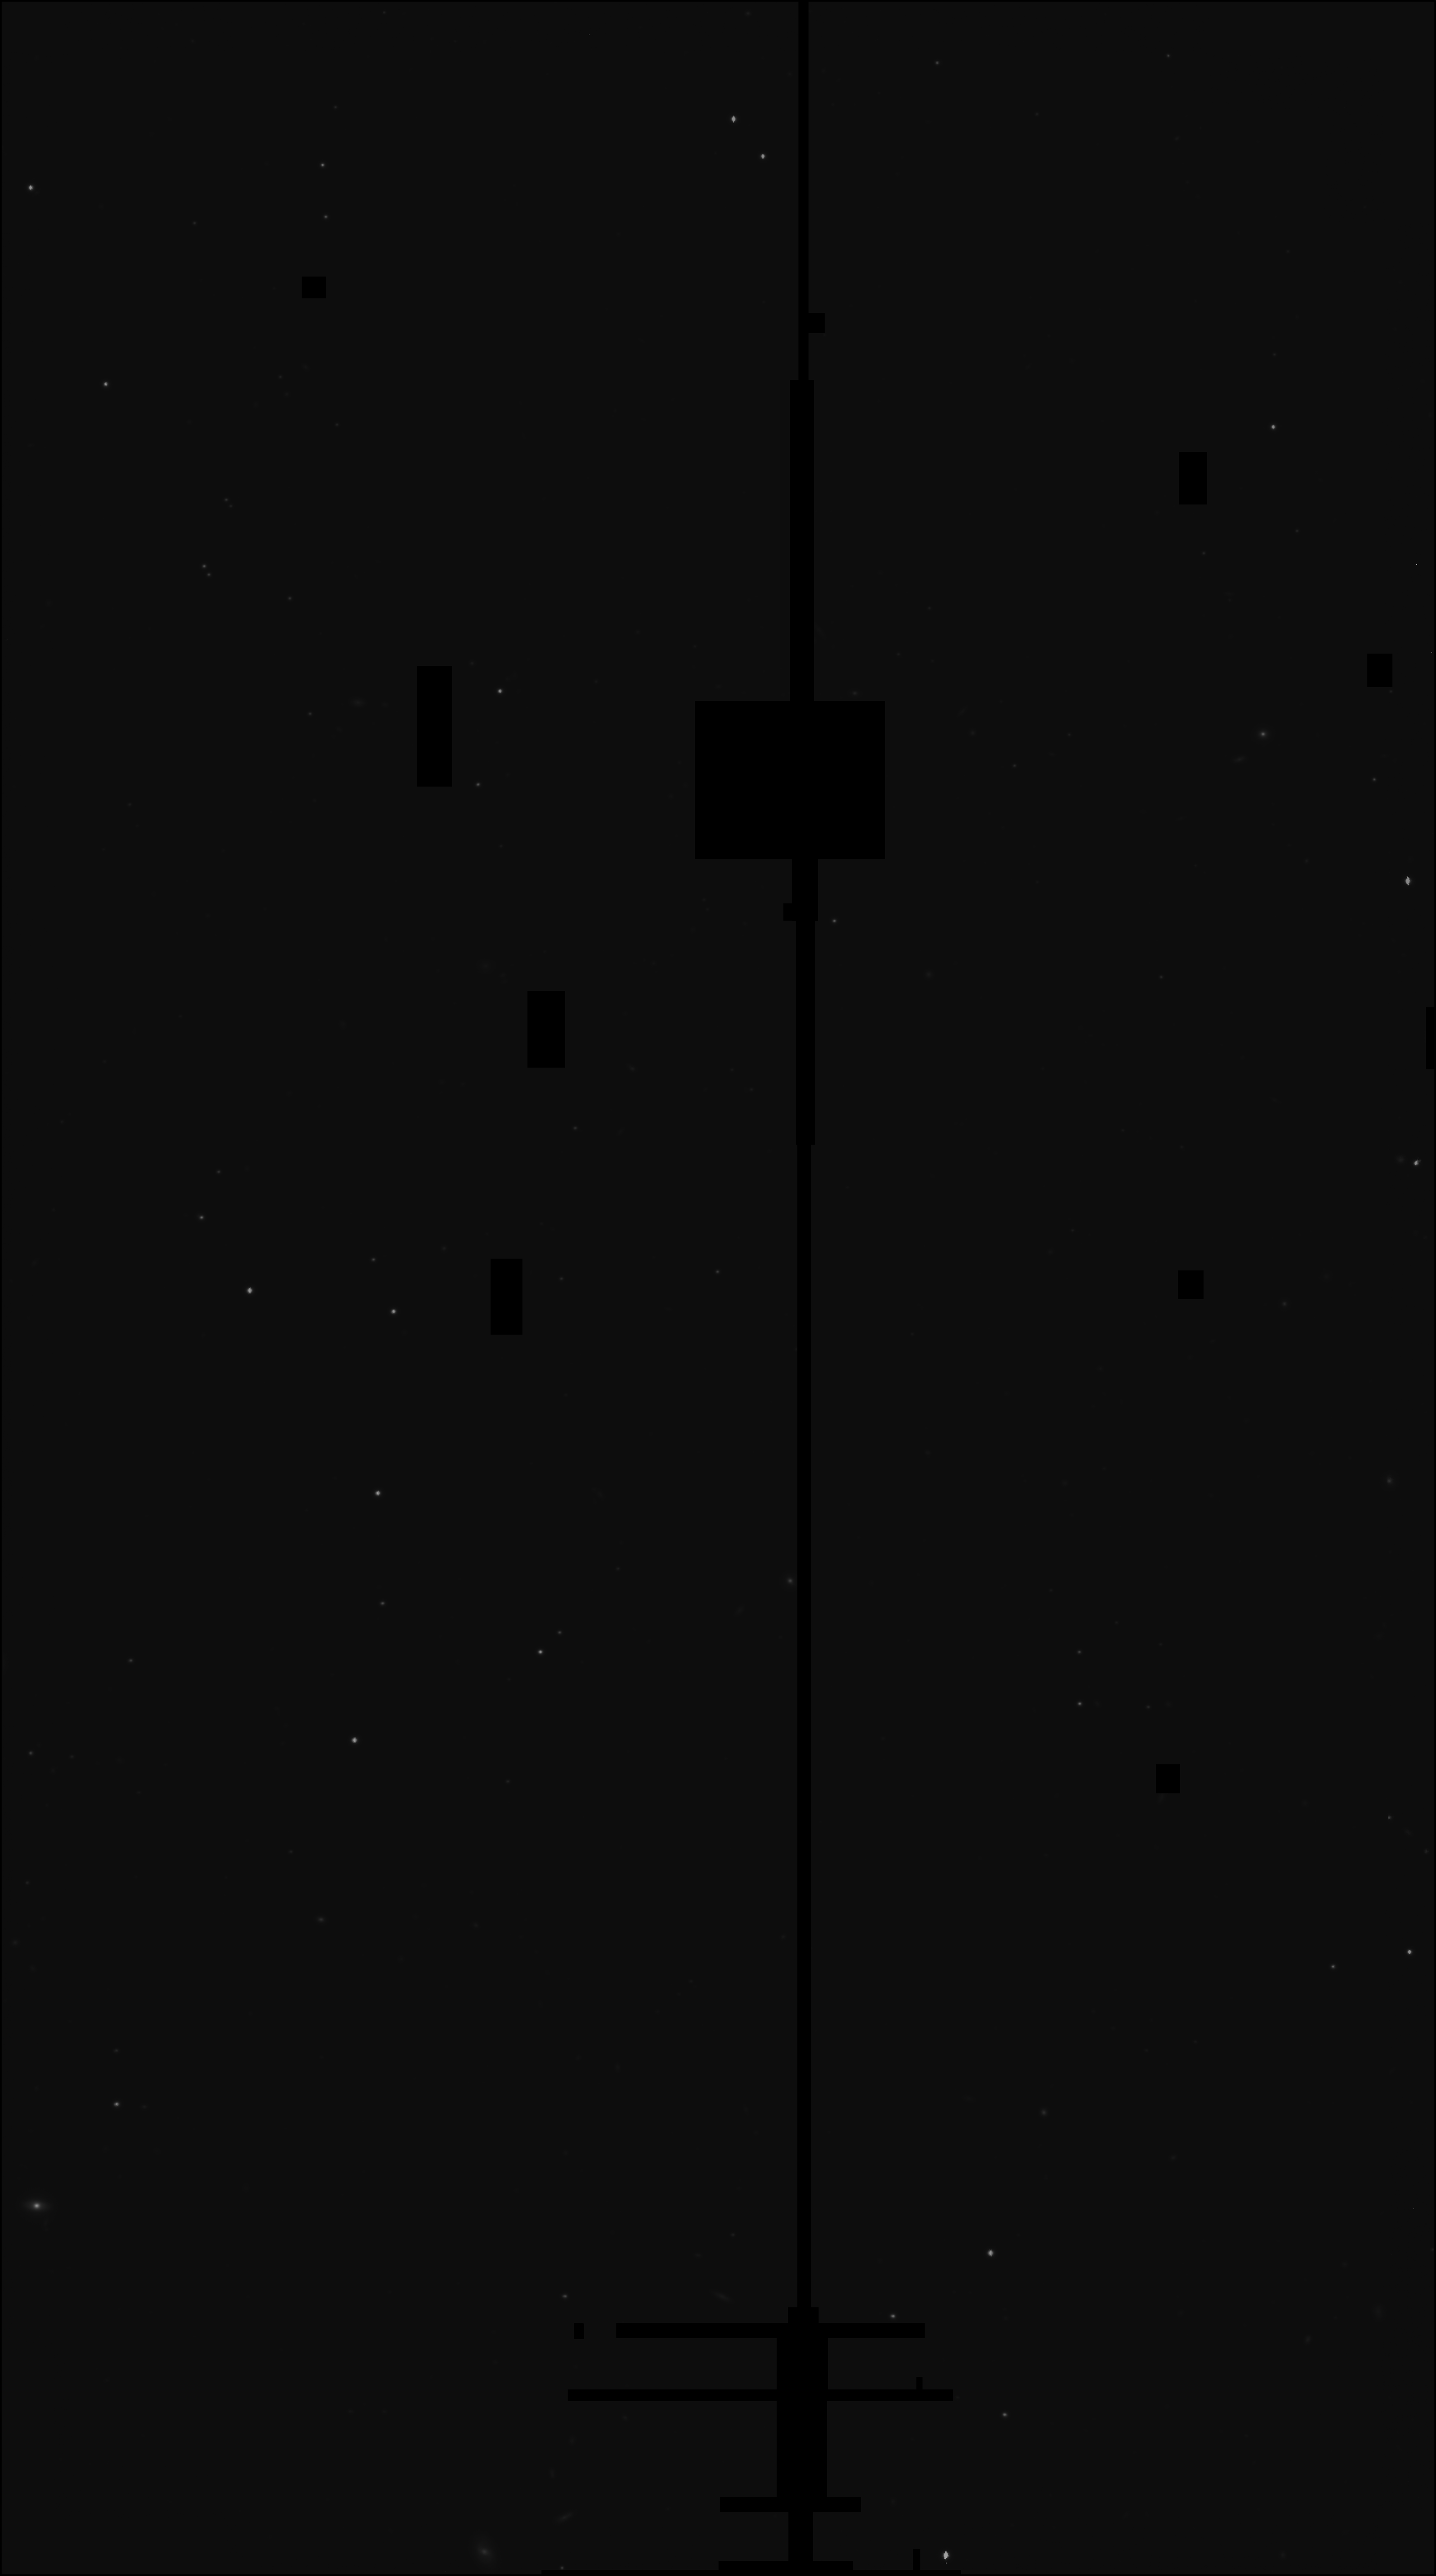
\includegraphics [width=5 cm]{mask.png}
\captionof{figure}{A copy of the original image with the masked "bad" regions removed.}
\label{mask}
\end{center}

\subsection*{Algorithms for Finding Galaxies}
Several methods were investigated to determine the aperture radius. The first method was to simply have a fixed aperture radius. The problem with this method was that if the aperture was too large multiple galaxies were counted as a single source. If the aperture was too small then a single large galaxy was counted as several galaxies. Therefore there was no ideal fixed aperture size and it was determined that a variable aperture was required. The first variable aperture method investigated was as follows. After the bright pixel at the center of the galaxy had been found counts of the pixels in eight directions were measured until the counts went below the minimum count. This gave eight possible radii. The largest was chosen to be the aperture radius. This method was quite successful apart from when there were two or more galaxies close together. When this happened the count did not go below the minimum until the radius covered several galaxies and they were counted as a single galaxy. A diagram showing a group of galaxies which caused this problem is shown in Figure \ref{algorithm1}. The first attempt to fix this was to limit the aperture radius to a maximum size. The problem with this is unless there isn't a radius that can be chosen that fixes all instances of this error and is still bigger than the biggest galaxy, If the maximum aperture size is smaller than the biggest galaxy then then it takes several apertures to cover a single galaxy as shown in Figure \ref{algorithm2}.

\begin{center}
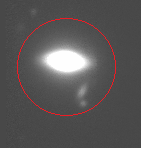
\includegraphics [width=10 cm]{algorithm1.png}
\captionof{figure}{Figure shows how two galaxies close together could be counted as one if the algorithm allows for large apertures. The aperture shown was not an aperture produced by the algorithm but is similar to apertures produced by the algorithm.}
\label{algorithm1}
\end{center}

\begin{center}
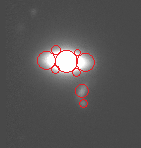
\includegraphics [width=10 cm]{algorithm2.png}
\captionof{figure}{Figure shows how a large galaxy could be counted as many if the algorithm is designed to not miss the smaller galaxy next to it. The apertures shown are not apertures produced by the algorithm but is similar to apertures produced by the algorithm.}
\label{algorithm2}
\end{center}


 To fix these problems a new algorithm was designed. Around the central bright pixel disks of counts were taken and averaged. The radius was chosen to be either when the average count of the disk went below the minimum count or when the count stopped decreasing at a rate which was determined experimentally.  

The average background count was taken from the galactic counts to give the true count of the galaxies. The use of local background counts was considered to take into account the varying background counts across the image but in the final data only a universal background was used for two main reasons. Firstly as shown by Figure \ref{hist} the local background count is normally distributed with a small standard deviation. The background count is 3423$\pm$26, this means the variation is about the mean is not significant compared to the galactic count as the variation is at most around 1\% of the count even for the faintest detectable galaxies. Further variation in the background flux could be caused by faint galaxies being detected next to bright sources . Taking local background counts was considered for this reason but when investigated it caused further issues. Local backgrounds were counted by counting pixels in a disk around the galaxy. Often this disk included other galaxies or stars. This made it possible for the disk to have a similar and sometimes greater average count than the galaxy itself. This made it possible for the algorithm to return galaxies with negative counts.


\section*{Results, Errors and Discussion}
The aim of the experiment was to measure the number and magnitude of galaxies within an image to catalogue them and see if they obeyed equation (\ref{eq:main}). Figure \ref{galaxy_counts} shows that the galaxy count does have a linear relationship on a logarithmic plot. The gradient is slightly different though to the gradient predicted by equation (\ref{eq:main}). The measured gradient is $0.650 \pm 0.002$ which is slightly different to 0.6. This could be due to a number of factors. The most significant factor is in this experiment only a small area of sky containing a relatively small number of galaxies was measured. For comparison there were 1455 galaxies found in the image used but there were 900,000 galaxies measured in the Sloan Digital Sky Survey \cite{paper}. The relationship described by equation (\ref{eq:main}) requires a large homogeneous sample of the sky. This is because on smaller local scales such as this one the homogeneousness of this area of the sky may not be complete. Further difference may be due to galaxy evolution. Due the finite speed of light looking at galaxies very far away is equivalent to looking at them in the past. In the distant past the flux produced by the galaxies may have been different which would contradict the assumption that the flux distribution of the galaxies is constant. The sample of galaxies in this survey is too small to determine if variations in the results are due to galaxy evolution of statistical variations.

The error in galaxy count is the square root of the count as the count obeys Poisson statistics. This means there is a more significant chance of there being less bright (low magnitude)  sources  than expected.  This is shown in the graph by the non-linear green part below a magnitude of around 10. The error on the galaxy count is the square root of the count as the counts are Poisson distributed.
\begin{center}
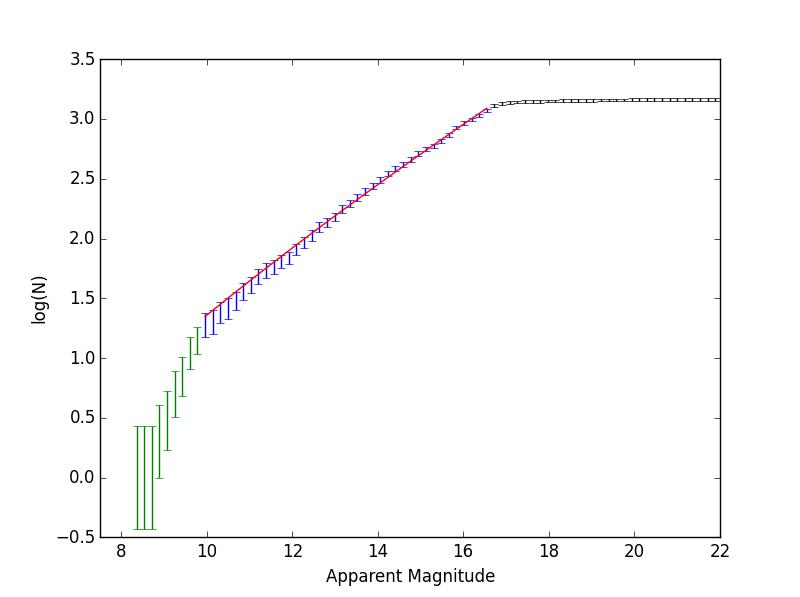
\includegraphics [width=10 cm]{graph.png}
\captionof{figure}{A plot of the log of the number of galaxies with an apparent magnitude m below m vs. apparent magnitude. The gradient of the straight section is $0.650\pm0.002$. The apparent magnitudes of the galaxies have been calculated relative to the AB magnitude system. }
\label{galaxy_counts}
\end{center}
The flattening of the graph above a magnitude of around 16  is due to incompleteness of the survey. As the galactic flux gets lower the chance of it being detected falls as it becomes indistinguishable from the background flux in the image. Eventually above a certain magnitude no further galaxies can be detected and the graph remains flat.

The catalogue produced contains among other information the location and magnitude of all 1455 galaxies found in the image. An extract from the catalogue is shown in Figure \ref{catalogue} in the appendix.

\section*{Conclusion}
A catalogue of 1455 galaxies was successfully produced. From the catalogue a graph of the number of galaxies vs absolute magnitude was produced. The gradient of the graph was similar but not in agreement within error to the predicted value. This is most likely to be due to the small sample of galaxies in this image. To achieve more consistent results a larger sample size of galaxies would be required such as in the  Sloan Digital Sky Survey \cite{paper}. The results could be further improved by improving the algorithm used to detect galaxies, for example by using elliptical apertures.

\bibliographystyle{unsrt}
\bibliography{Bibliography}

\section*{Appendix}
\subsection*{Derivation of Equation (\ref{eq:main})}

The derivation assumes the galaxies are uniformly distributed in space so the number of galaxies $N(r)$ in a given radius is:
\begin{equation}\label{N(r)}
N(r) = \frac{4}{3} \pi r^3 \rho
\end{equation}
where $\rho$ is the density of galaxies. Magnitudes are always measured against a reference flux $f_R$. Magnitudes are given by:
\begin{equation}\label{m}
m = -2.5 \log(\frac{f}{f_R})
\end{equation}
where $f$ is the flux received from the galaxy. As the flux distribution is assumed to be fixed the expectation value the total flux produced by a galaxy $f_G$ is constant. The flux $f$ is given by:
\begin{equation}\label{f}
f = \frac{f_G}{r^2}
\end{equation}
Therefore by subbing (\ref{f}) into (\ref{m}):
\begin{equation}
m = -2.5\log(\frac{f_G}{f_R r^2})
\end{equation}
\begin{equation}
m = 5\log(r)-2.5\log(\frac{f_G}{f_R})
\end{equation}
\begin{equation}\label{m,r}
m = 5\log(r) + c'
\end{equation}
where $c' = -2.5\log(\frac{f_G}{f_R})$ is a constant. Rearranging (\ref{m,r}): 
\begin{equation}\label{r}
r = 10^{\frac{m}{5}-c'}
\end{equation}
Then subbing (\ref{r}) into (\ref{N(r)}):
\begin{equation}
N(m) = \frac{4}{3} \pi 10^{\frac{3m}{5}-3c'} \rho
\end{equation}
Then taking the $\log$:
\begin{equation}
\log(N(m)) = \log(\frac{4}{3} \pi 10^{\frac{3m}{5}-3c'} \rho)
\end{equation}
\begin{equation}
\log(N(m)) = \log(10^{\frac{3m}{5}-3c'}) + \log(\frac{4}{3} \pi \rho)
\end{equation}
\begin{equation}
\log(N(m)) = \frac{3m}{5}-3c' + \log(\frac{4}{3} \pi \rho)
\end{equation}
\begin{equation}\label{eq:final}
\log(N(m)) = 0.6m+ c
\end{equation}
where $c = -3c' + \log(\frac{4}{3} \pi \rho)$  is a constant. Equation (\ref{eq:final}) is identical to equation (\ref{eq:main}) as required.

\verbatiminput{catalog.txt}\captionof{figure}{A sample of the galaxy catalogue produced. Radii are in units of pixels.}\label{catalogue}

\end{document}
